% !TEX root =../ECE343_Slides_Rogers.tex

\section{Schedule}
\renewcommand{\arraystretch}{1}
\begin{frame}{Nominal Schedule}
	\begin{textblock}{13}(0.5,2.15)
	\def\myfontsize{footnotesize}
	\newcounter{mylnum}
	\def\lessonNum{1}
%	\setcounter{mylnum}{1}
	
\setcounter{mylnum}{1}
\begin{center}
\begin{\myfontsize}
\begin{tabular}{| c | l | c | l |}
\hline
\textbf{Lesson} 		  	& \textbf{Topics}             & \pbox{5cm}{\textbf{Reading}}	& \textbf{Notes}		\\ \hline\hline
\ifnum\lessonNum=\value{mylnum} \rowcolor{green!20!white}\fi
	\themylnum  
	& Course Overview  \& Introduction		
	& Ch.1 
	&  LO 1.1-1.2 
	\stepcounter{mylnum}\\ \hline \hline
\rowcolor{gray!20!white}\multicolumn{4}{| c |}{\textbf{Chapter 2: Electric and Magnetic Fields}}	\\ \hline\hline
\ifnum\lessonNum=\value{mylnum} \rowcolor{green!20!white}\fi
	\themylnum 	
	& Fields, Parameters, Field Quantities	
	& Ch. 2	
	& LO 2.1-2.2			
\stepcounter{mylnum}\\ \hline\hline
\rowcolor{gray!20!white}\multicolumn{4}{| c |}{\textbf{Chapter 3: Transmission Lines}}	 \\ \hline\hline	
\ifnum\lessonNum=\value{mylnum} \rowcolor{green!20!white}\fi
	\themylnum 	
	& Lumped Element Model				
	& 3.1-3.4 
	& LO 3.1		
\stepcounter{mylnum}\\ \hline
\ifnum\lessonNum=\value{mylnum} \rowcolor{green!20!white}\fi
	\themylnum 	
	& Telegrapher's Equations
	& 3.5-3.6
	&  LO 3.1	
\stepcounter{mylnum}\\ \hline
\ifnum\lessonNum=\value{mylnum} \rowcolor{green!20!white}\fi
	\themylnum 	
	&  Characteristic Impedance \& Wave Propagation	
	& 3.7-3.9		
	& LO 3.2						
\stepcounter{mylnum}\\ \hline
\ifnum\lessonNum=\value{mylnum} \rowcolor{green!20!white}\fi
	\themylnum 	
	& Coaxial,  Reflection Coefficient, VSWR	
	& 3.10,3.12-3.14	
	& LO 3.2-3.3		
\stepcounter{mylnum}\\ \hline 
\ifnum\lessonNum=\value{mylnum} \rowcolor{green!20!white}\fi
	\themylnum 	
	&  Terminated Transmission Lines	
	&  3.15,3.17-3.19
	& LO 3.4		
\stepcounter{mylnum}\\ \hline 
\ifnum\lessonNum=\value{mylnum} \rowcolor{green!20!white}\fi
	\themylnum	
	& Impedance Matching	
	& 3.21-3.23
	& LO 3.4 			
\stepcounter{mylnum}\\ \hline 
\ifnum\lessonNum=\value{mylnum} \rowcolor{green!20!white}\fi
	\themylnum  
	& Impedance Matching	
	& 3.21-3.23
	& LO 3.4		
\stepcounter{mylnum}\\ \hline 
\ifnum\lessonNum=\value{mylnum} \rowcolor{green!20!white}\fi
	\themylnum	
	& Smith Charts
	& Supplemental
	& LO 3.5
\stepcounter{mylnum}\\ \hline 
\ifnum\lessonNum=\value{mylnum} \rowcolor{green!20!white}\fi
	\themylnum	
	& Smith Charts
	& Supplemental 
	& LO 3.5					
\stepcounter{mylnum}\\ \hline 
\ifnum\lessonNum=\value{mylnum} \rowcolor{green!20!white}\fi
	\themylnum	
	& Smith Charts
	& Supplemental 
	& LO 3.5	
\stepcounter{mylnum}\\ \hline 
\ifnum\lessonNum=\value{mylnum} \rowcolor{green!20!white}\fi
	\themylnum	
	& Smith Charts
	& Supplemental 
	& LO 3.5	
\stepcounter{mylnum}\\ \hline 

\ifnum\lessonNum=\value{mylnum} \rowcolor{green!20!white}\fi
	\themylnum	
	& Transients		
	& Supplemental 
	& LO 3.6	 
\stepcounter{mylnum}\\ \hline \hline
\ifnum\lessonNum=\value{mylnum} \rowcolor{green!20!white}\fi
	\themylnum 	
	& Flex Day
	& 
	& 	
\stepcounter{mylnum}\\ \hline 
\ifnum\lessonNum=\value{mylnum} \rowcolor{green!20!white}\fi
	\themylnum 	
	& Reflection/Transmission Coefficient Lab
	& Lab Packet
	& LO 3.7		
\stepcounter{mylnum}\\ \hline 
\ifnum\lessonNum=\value{mylnum} \rowcolor{green!20!white}\fi
	\themylnum 	
	& Reflection/Transmission Coefficient Lab
	& Lab Packet
	& LO 3.7		
\stepcounter{mylnum}\\ \hline 
\rowcolor{gray!20!white}\multicolumn{4}{| c |}{\textbf{Chapter 4: Vector Analysis}} \\ \hline\hline
\ifnum\lessonNum=\value{mylnum} \rowcolor{green!20!white}\fi
	\themylnum	
	& Vector \& Coordinate System Review
	& Ch. 4
	&LO 4.1-4.4 \textbf{GR 1 due}	
\stepcounter{mylnum}\\ \hline 
\rowcolor{gray!20!white}\multicolumn{4}{| c |}{\textbf{Chapter 5: Electrostatics}}\\ \hline\hline
\ifnum\lessonNum=\value{mylnum} \rowcolor{green!20!white}\fi
	\themylnum	
	& Coulomb's Law
	& 5.1-5.3
	& LO 5.1
\stepcounter{mylnum}\\ \hline 
\ifnum\lessonNum=\value{mylnum} \rowcolor{green!20!white}\fi
	\themylnum	
	& Surface and Volume Charge			
	& 5.4
	& LO 5.1
\stepcounter{mylnum}\\ \hline 
\ifnum\lessonNum=\value{mylnum} \rowcolor{green!20!white}\fi
	\themylnum	
	& Gauss' Law (Integral Form)
	& 5.5-5.6
	& LO 5.2		 					
\stepcounter{mylnum}\\ \hline 
\ifnum\lessonNum=\value{mylnum} \rowcolor{green!20!white}\fi
	\themylnum	
	& Gauss' Law (Differential Form)		
	& 5.7-5.8
	& LO 5.2	 	
\stepcounter{mylnum}\\ \hline 
\ifnum\lessonNum=\value{mylnum} \rowcolor{green!20!white}\fi
	\themylnum	
	& Electric Potential	
	& 5.9-5.10, 5.15
	&  LO 5.3	
\stepcounter{mylnum}\\ \hline 
% <---- line 129 should be 20 lessons, based on 6 lines per lesson, starting at line 9 
\end{tabular}			
\end{\myfontsize}
\end{center}

	\end{textblock}
\end{frame}

%%%%%%%%%%%%%%%%%%%%%%%%%%%%%%%%%%%%%%%%%%%%%%%%%%%%%
%%%%%%%%%%%%%%%%%%%%%%%%%%%%%%%%%%%%%%%%%%%%%%%%%%%%%

\begin{frame}{Ch 1 Learning Objectives}
	\begin{textblock}{14}(0.5,5)
		\begin{enumerate}[{1}.1]
			\setlength{\itemsep}{18pt}
			\item I can articulate what I will learn and how I will be assessed in this course.
			\item<alert> I can articulate practical applications of electromagnetics.
		\end{enumerate}
	\end{textblock}
\end{frame}
%%%%%%%%%%%%%%%%%%%%%%%%%%%%%%%%%%%%%%%%%%
%%%%%%%%%%%%%%%%%%%%%%%%%%%%%%%%%%%%%%%%%%

\begin{frame}{The Story of Energy \& Waves}
	\begin{textblock}{14.5}(0.5,3)
	 Read. The. \href{https://usafa0.sharepoint.com/:f:/s/ECE343-Spring2024/Et2Y5hmFiwlEiXtiAGOJz4EBd4ZjSs43FW_9L7Wvh8H4QA?e=EOZfAW}{Book}:
	\begin{itemize}
		\setlength\itemsep{12pt}
			\item Chapter 2 - Fields
			\item Chapter 3 - Transmission Lines
			\item Chapter 4 - Vector Analysis
			\item Chapter 5 - Electrostatics
			\item Chapter 6 - Current \& Conductivity
			\item Chapter 7 - Magnetostatics
			\item Chapter 8 - Dynamic Fields
			\item Chapter 9 - Plane Waves
	\end{itemize}
	\end{textblock}
	
	\begin{textblock}{6}(9.5,6)
	
	\includegraphics[scale=0.23]{ECE343/officespace}
	
	\end{textblock}
\note{}
\end{frame}

%%%%%%%%%%%%%%%%%%%%%%%%%%%%%%%%%%%%%%%%%%%%%%%%%%%%%
%%%%%%%%%%%%%%%%%%%%%%%%%%%%%%%%%%%%%%%%%%%%%%%%%%%%%

%%%%%%%%%%%%%%%%%%%%%%%%%%%%%%%%%%%%%%%%%%%%%%%%%%%%%
%%%%%%%%%%%%%%%%%%%%%%%%%%%%%%%%%%%%%%%%%%%%%%%%%%%%%

\begin{frame}{Maxwell's Equations}

\begin{textblock}{8}(0.5,3.5)
\renewcommand{\arraystretch}{2.5}
\begin{tabular}{| c | c | c |}
\hline
			& Integral Form & Differential Form \\ \hline\hline
Gauss	& ${\displaystyle \oint \vec{E}\mycdot \vec{dS}} = Q_{\text{enc}} $ & $\nabla\mycdot\vec{E}  = \dfrac{\rho_v}{\epsilon}$   \\ \hline
Gauss  & ${\displaystyle\oint \vec{H}\mycdot\vec{dS} } = 0 $ & $\nabla\mycdot\vec{H} = 0$ \\ \hline
Faraday & ${\displaystyle\oint_C \vec{E}\mycdot d\ell = -\mu\int\partd{\vec{H}}{t}\mycdot \vec{dS}}$& $\nabla\times\vec{E} = -\mu\partd{\vec{H}}{t}$ \\ \hline
Ampere 	& ${\displaystyle\oint_C\vec{H}\mycdot d\ell = \int \vec{J}\mycdot\vec{dS} + \epsilon\partd{}{t}\int\vec{E}\mycdot\vec{dS}}$ & $\nabla\times\vec{H} = \vec{J}_C + \epsilon\partd{\vec{E}}{t}$ \\ \hline
\end{tabular}
\end{textblock}


\end{frame}

%%%%%%%%%%%%%%%%%%%%%%%%%%%%%%%%%%%%%%%%%%%%%%%%%%%%%
%%%%%%%%%%%%%%%%%%%%%%%%%%%%%%%%%%%%%%%%%%%%%%%%%%%%%

\begin{frame}{Ampere's Force Law - Parallel Wires}

\begin{textblock}{14.5}(1,4.5)

%	\input{./figures/ampere_wire_attraction}
\includegraphics[scale=1]{ECE343/ampere_current_attract}

\end{textblock}


\end{frame}

%%%%%%%%%%%%%%%%%%%%%%%%%%%%%%%%%%%%%%%%%%%%%%%%%%%%%
%%%%%%%%%%%%%%%%%%%%%%%%%%%%%%%%%%%%%%%%%%%%%%%%%%%%%

\begin{frame}{Ampere's Force Law}

\begin{textblock}{8}(0.5,3.5)
	\includegraphics[scale=0.75]{ECE343/MotorTheory}
\end{textblock}


\end{frame}

%%%%%%%%%%%%%%%%%%%%%%%%%%%%%%%%%%%%%%%%%%%%%%%%%%%%%
%%%%%%%%%%%%%%%%%%%%%%%%%%%%%%%%%%%%%%%%%%%%%%%%%%%%%

\begin{frame}{Faraday's Law \& KVL}

\begin{textblock}{14.5}(0.5,3)
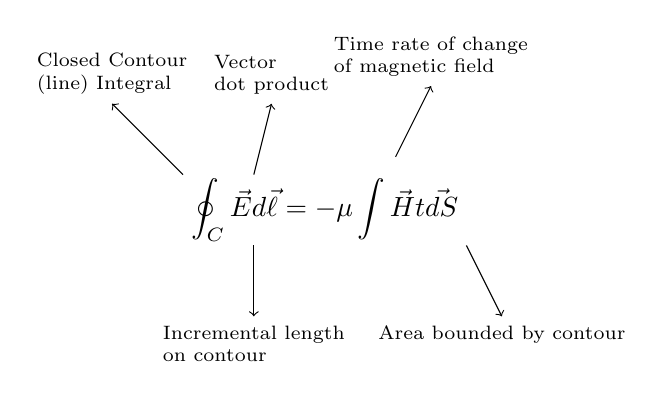
\begin{tikzpicture}[scale=0.9]
\node at (0,0) {
	$
		{\displaystyle\oint_C \vec{E}\mycdot d\vec{\ell} = -\mu\int\partd{\vec{H}}{t}\mycdot \vec{dS}}
		$
	};
	\draw[->] (-2,0.5) --++ (-1,1) node[above, font={\scriptsize}, align=left] {Closed Contour \\ (line) Integral};
	\draw[->] (-1,0.5) --++ (0.25,1) node[above, font={\scriptsize}, align=left] {Vector \\ dot product};
	\draw[->] (-1,-0.5) --++ (0,-1) node[below,  font={\scriptsize}, align=left] {Incremental length \\ on contour};
	\draw[->] (1,0.75) --++ (0.5,1) node[above,  font={\scriptsize}, align=left] {Time rate of change \\ of magnetic field};
	\draw[->] (2,-0.5) --++ (0.5,-1) node[below,  font={\scriptsize}, align=left] {Area bounded by contour};
\end{tikzpicture}
\end{textblock}

\begin{textblock}{14.5}(1,10.5)

\begin{circuitikz}
	
	\draw (0,0) to[sV] ++(0,2)
				to[R=R] ++(2,0)
				to[twoport, a=Z] ++(0,-2)
				to[short] (0,0);

\end{circuitikz}

\end{textblock}

\begin{textblock}{14.5}(8,10.5)

\begin{circuitikz}
	
	\draw (0,0) to[sV] ++(0,2)
				to[R=R] ++(2,0)
				to[twoport, a=Z] ++(0,-2)
				to[short] (0,0);

\end{circuitikz}

\end{textblock}

\end{frame}

%%%%%%%%%%%%%%%%%%%%%%%%%%%%%%%%%%%%%%%%%%%%%%%%%%%%%
%%%%%%%%%%%%%%%%%%%%%%%%%%%%%%%%%%%%%%%%%%%%%%%%%%%%%

\begin{frame}{Current Continuity \& KCL}
			\begin{textblock}{14.5}(0.5,3)
			\eq{
				\nabla\mycdot\vec{J} = -\partd{\rho_V}{t}
			}
				\begin{tikzpicture}
					\draw[black, thick] (0,6) --++ (10,0);
					\draw[black, thick] (0,4) --++ (4,0);
					 \draw[black, thick] (6,4) --++ (4,0);
					 \draw[black, thick] (4,0) --++(0,4);
					 \draw[black, thick] (6,0) --++(0,4);
				\end{tikzpicture}
			\end{textblock}
\end{frame}

%%%%%%%%%%%%%%%%%%%%%%%%%%%%%%%%%%%%%%%%%%%%%%%%%%%%%
%%%%%%%%%%%%%%%%%%%%%%%%%%%%%%%%%%%%%%%%%%%%%%%%%%%%%

\begin{frame}{Emag Demos}

\begin{textblock}{8}(0.5,3)
	\href{https://www.youtube.com/watch?v=lY6XCmPjqyA}{\includegraphics[scale=0.25]{ECE343/oersted}}
\end{textblock}

\begin{textblock}{8}(0.5,9)
	\href{https://www.youtube.com/watch?v=_k0JJpJ4_sw}{\includegraphics[scale=0.25]{ECE343/induction}}
\end{textblock}

\begin{textblock}{8}(10.5,3.5)
	\href{https://www.youtube.com/watch?v=oZZYZ61AMhg}{\includegraphics[scale=0.07]{ECE343/teslacoil}}
\end{textblock}

\begin{textblock}{8}(10.5,9)	
	\href{https://www.youtube.com/watch?v=r1Tuh9wUP0g}{\includegraphics[scale=0.1]{ECE343/sparkplug}}
\end{textblock}

\end{frame}


%%%%%%%%%%%%%%%%%%%%%%%%%%%%%%%%%%%%%%%%%%%%%%%%%%%%%
%%%%%%%%%%%%%%%%%%%%%%%%%%%%%%%%%%%%%%%%%%%%%%%%%%%%%

\begin{frame}{Preliminary Concepts - Spectrum}

\begin{textblock}{16}(0,0)
	\includegraphics[width=\textwidth, height=9.75cm]{ECE343/Emag_characteristics}
\end{textblock}
\end{frame}


%%%%%%%%%%%%%%%%%%%%%%%%%%%%%%%%%%%%%%%%%%%%%%%%%%%%%
%%%%%%%%%%%%%%%%%%%%%%%%%%%%%%%%%%%%%%%%%%%%%%%%%%%%%

%\begin{frame}{KVL - DC excitation}
%		\begin{textblock}{14.5}(0.5,3)
%			\begin{circuitikz}
%				\draw (0,0) to[V,a^=1V, invert] ++(0,2)
%									to[R=100\ohms] ++(0,2)
%									to[short] ++(4,0)
%									to[R=900\ohms] ++(0,-4)
%									to[short] ++(-4,0);
%			\node at (2,4.5) {A};
%			\node at (2,-0.5) {B};
%			\end{circuitikz}
%		\end{textblock}
%\end{frame}
%
%%%%%%%%%%%%%%%%%%%%%%%%%%%%%%%%%%%%%%%%%%%%%%%%%%%%%
%%%%%%%%%%%%%%%%%%%%%%%%%%%%%%%%%%%%%%%%%%%%%%%%%%%%%
%
%\begin{frame}{KVL - Solenoid Excitation}
%		\begin{textblock}{14.5}(0.5,3)
%			\begin{circuitikz}
%				\draw (0,0) to[short] ++(0,2)
%									to[R=100\ohms] ++(0,2)
%									to[short] ++(4,0)
%									to[R=900\ohms] ++(0,-4)
%									to[short] ++(-4,0);
%			\node at (2,4.5) {A};
%			\node at (2,-0.5) {B};
%			\end{circuitikz}
%		\end{textblock}
%\end{frame}
%
%%%%%%%%%%%%%%%%%%%%%%%%%%%%%%%%%%%%%%%%%%%%%%%%%%%%%
%%%%%%%%%%%%%%%%%%%%%%%%%%%%%%%%%%%%%%%%%%%%%%%%%%%%%
%
%\begin{frame}{KVL - AC Excitation}
%		\begin{textblock}{14.5}(0.5,3)
%			\begin{circuitikz}
%				\draw (0,0) to[vco,a^=\myv{0}\cos{\omega t}, invert] ++(0,2)
%									to[R=100\ohms] ++(0,2)
%									to[short] ++(4,0)
%									to[R=900\ohms] ++(0,-4)
%									to[short] ++(-4,0);
%			\node at (2,4.5) {A};
%			\node at (2,-0.5) {B};
%			\end{circuitikz}
%		\end{textblock}
%\end{frame}


